\section{Delegating Computation and the GKR Protocol (Incomplete)}

Until now we have considered interactive proofs with a polynomial time verifier. While the formal definition of IPs allows the prover to have unbounded computational power, we often consider situations in which the honest prover also works efficiently.

Suppose we are given a boolean formula $\phi=\phi(x_1,\dots,x_n)$. Then,
\begin{itemize}
	\item in the sumcheck protocol for $\#\mathsf{SAT}$, the prover takes time $\Omega(2^n|\phi|)$, since it has to sum over all possible values of $(x_1,\dots,x_n)$.
	\item in Shamir's protocol for $\mathsf{TQBF}$, the prover similarly has to take time $\Omega(2^n|\phi|)$.
\end{itemize}

These times are too high to be practically useful for computation. Suppose we have a machine $M$ that runs in time $T$ and in space $S$. Then, we can reduce the language $L_m=\{x:M(x)=1\}$ to a $\mathsf{TQBF}$ instance $\phi(x_1,\dots,x_n)$, where $$n\geq \log{T}\cdot S$$ Even if both $T,S\in\poly(n)$, it follows that the prover time is $\Omega(2^n)=\Omega(T^S)=n^{\omega(1)}$.

\subsection{Doubly-Efficient Interactive Proofs}

\begin{definition}[Doubly-Efficient Interactive Proof]
	A deIP is an interactive proof in which the prover is additionally constrained to run in polynomial time.
\end{definition}

Intuitively, deIPs are interactive proofs which are `computationally useful,' ie. can be used to delegate computation. These are particularly useful when the verifier requires less resources to run than calculating the proof itself -- for instance, instead of performing a heavy $O(n^6)$ algorithm, the verifier can delegate the task to the prover and simply check the solution using only $O(n)$ or $O(n\log n)$ time. In special cases, the prover may even need to run for time sublinear in the problem length.

We now give a first characterization of $\mathbf{deIP}$.

\begin{theorem}
	$\mathbf{deIP}\subseteq\mathbf{BPP}$.
	\label{thm:deip}
\end{theorem}
\begin{proof}
	The probabilistic algorithm simply simulates the interaction between prover and verifier, which it can do in polynomial time and using the verifier's randomness.
\end{proof}

\subsection{Delegation for Bounded-Depth Circuits}

\begin{definition}[$S$-Space Uniform Circuit Family]
	A circuit family $\mathcal{C}_i=\{C\}_{i\in\mathbb{N}}$ is $S$-space uniform if there exists a machine $M$ such that $M(1^n)=C_n$ and $M$ runs in space $O(S(n))$.
\end{definition}

We now see a theorem that relates $\ip$ and languages decidable by circuits.

\begin{theorem}
	Suppose that $L$ is decidable by an $O(\log S)$-space uniform circuit family of size $S$ and depth $D$. Then $L$ has a public coin IP such that
	\begin{itemize}
		\item the prover time is $\poly(S)$,
		\item the verifier time is $(n+D)\cdot\mathsf{polylog}(S)$ and space is $O(\log S)$,
		\item the total communication is $D\cdot\mathsf{polylog}(S)$.
	\end{itemize}
\end{theorem}

The proof of this theorem is long and technical. We will see only the bare-bones protocol, in which the verifier has query access to the circuit's topology. We will thus not need to discuss uniformity.

The protocol we will discuss is called the GKR protocol and is highly efficient in practice. \cite{10.1145/2699436} was introduced by Goldwasser, Kalai and Rothblum in 2008 and uses ideas of arithmetization and sumcheck. Furthermore, GKR can be modified so that the prover runs in linear time, and the verifier can in fact verify the computation using time sublinear in the size of the circuit.

GKR is also interesting in terms of providing an IP for the circuit complexity class $\mathbf{NC}$. Using GKR yields a polytime prover and a linear time verifier.

\subsubsection{Layered Arithmetic Circuits}

\begin{definition}[Layered Arithmetic Circuit]
	An arithmetic circuit $C:\F^n\rightarrow\F$ of size $S$, depth $D$ and fan-in $2$ arranged in $D+1$ layers.
\end{definition}

\begin{figure}[h]
	\begin{center}
		{\renewcommand{\arraystretch}{1.2}%
		\begin{tabular}{ c c c }
			\hline
			\multirow{2}{6em}{Layer $0$} & \multirow{2}{6em}{$V_0\in\F$} & \\
			&&\\
			\hline
			\multirow{2}{6em}{Layer $1$} & \multirow{2}{6em}{$V_1:S\rightarrow\F$} & $\add_1:[S]^3\rightarrow\{0,1\}$ \\ 
			& & $\mul_1:[S]^3\rightarrow\{0,1\}$ \\
			\hline
			\multirow{2}{6em}{Layer $2$} & \multirow{2}{6em}{$V_2:S\rightarrow\F$} & $\add_2:[S]^3\rightarrow\{0,1\}$ \\ 
			& & $\mul_2:[S]^3\rightarrow\{0,1\}$ \\
			\hline
			\vdots & \vdots & \vdots \\
			\hline
			\multirow{2}{6em}{Layer $D-1$} & \multirow{2}{6em}{$V_{D-1}:S\rightarrow\F$} & $\add_{D-1}:[S]^3\rightarrow\{0,1\}$ \\ 
			& & $\mul_{D-1}:[S]^3\rightarrow\{0,1\}$ \\ 
			\hline
			\multirow{2}{6em}{Layer $D$} & \multirow{2}{6em}{$V_D:S\rightarrow\F$} & $\add_D:[S]\times [n]^2\rightarrow\{0,1\}$ \\ 
			& & $\mul_D:[S]\times[n]^2\rightarrow\{0,1\}$ \\
			\hline
		\end{tabular}
	}
	\end{center}
	\caption{A Layered Circuit.}
	\label{fig:layeredcircuit}
\end{figure}

Figure \ref{fig:layeredcircuit} gives a functional representation of a layered circuit. At each level are gates, which contain either $+$ or $\times$ and represent the sum or product of the input wires into the gate. We can additionally define two functions $\add_i$ and $\mul_i$.
\begin{align*}
	\add_i(g_j,w_k,w_l)=
	\begin{cases}
		1&\text{if $g_i$ is a $+$ gate with input wires from nodes $w_k$ and $w_l$,}\\
		0&\text{otherwise.}
	\end{cases}
\end{align*}
\begin{align*}
	\mul_i(g_j,w_k,w_l)=
	\begin{cases}
		1&\text{if $g_i$ is a $\times$ gate with input wires from nodes $w_k$ and $w_l$,}\\
		0&\text{otherwise.}
	\end{cases}
\end{align*}

$\add$ and $\mul$ are called \textit{wiring predicates}. For notational simplicity, we assume that $C$ has only one kind of gate, $g:\F^n\rightarrow F$.

\begin{figure}[h]
	\centering
	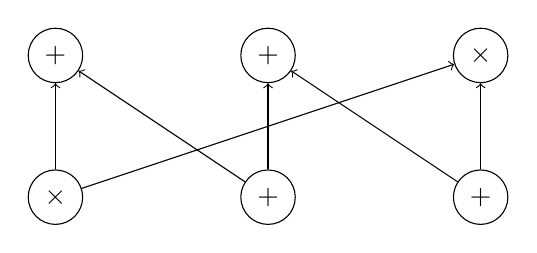
\begin{tikzpicture}  
		[scale=.9,auto=center,every node/.style={circle,draw}] % here, node/.style is the style pre-defined, that will be the default layout of all the nodes. You can also create different forms for different nodes.  
		
		\node (a1) at (0,1) {$+$};  
		\node (a2) at (-3,1)  {$+$}; 
		\node (a3) at (3,1)  {$\times$};  
		\node (a4) at (0,-1) {$+$};  
		\node (a5) at (-3,-1)  {$\times$};  
		\node (a6) at (3,-1)  {$+$};   
		
		\draw [<-] (a1) -- (a4);
		\draw [<-] (a1) -- (a6);
		\draw [<-] (a2) -- (a5);
		\draw [<-] (a2) -- (a4);
		\draw [<-] (a3) -- (a5);
		\draw [<-] (a3) -- (a6);
		
	\end{tikzpicture}  
	\caption{Two Layers of a Circuit.}
\end{figure}

\subsubsection{Low-Degree Extensions}

\begin{definition}[Polynomial Extension]
	Let $H\subseteq\F$ be a domain and $f:H\rightarrow\F$ be a function. Then a polynomial $p\in\F[x]$ is called an extension of $f$ if $p|_H=f$.
\end{definition}

We are interested in low-degree extensions, in which the polynomial has a low degree. The lowest degree (or minimal) extension is the extension obtained through Lagrange Interpolation: the degree is $<|H|$, and can be calculated as
$$p(x)=\sum_{\alpha\in H}f(\alpha)\left[\prod_{\beta\in H\setminus\{\alpha\}}\left(\frac{x-\beta}{\alpha-\beta}\right)\right]$$

The term in the square braces is called the Lagrange polynomial, and we represent it as $L_{\alpha,H}(x)$. We can easily extend this to the multivariate case. It follows that
\begin{itemize}
	\item $p\in\F[x_1,\dots,x_n]$ extends $f:H^n\rightarrow\F$ if $p|_{H^n}=f$.
	\item the extension of minimum degree has individual degree $<|H|$ and equals
	 $$p(x_1,\dots,x_n)=\sum_{\alpha_1,\dots,\alpha_n\in H}f(\alpha_1,\dots,\alpha_n)\left(\prod_{\alpha_i}L_{\alpha_i,H}\right)$$
	 where the product of the lagrange polynomials is the multivariate lagrange polynomial $L_{\alpha_1\dots,\alpha_n, H^n}$.
\end{itemize}

\subsubsection{Layer Arithmetization}
